\section{Uživatelské rozhraní}


\subsection{Domovská stránka}
Návrh domovské (obrázek \ref{wireframe-hlavni}) stránky je velmi minimalistický. Stránka slouží pouze k~seznámení uživatele s~významem aplikace a k~navigaci na další stránky pomocí dvou velkých bloků umístěných pod úvodní fotografií.

\begin{figure}[htbp]
    \centering
    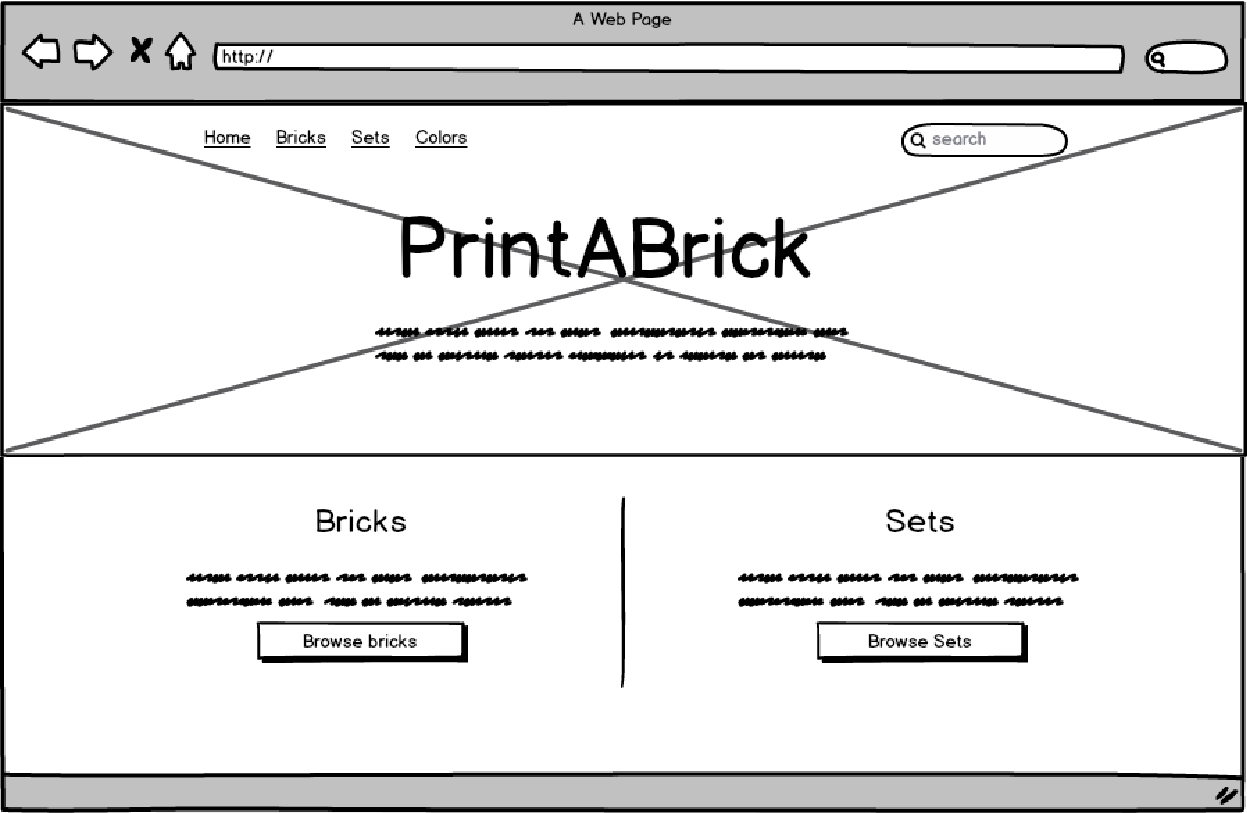
\includegraphics[width=\textwidth,height=\textheight,keepaspectratio]{pdfs/wireframe_home.pdf}
    \caption{Návrh hlavní stránky}\label{wireframe-hlavni}
\end{figure}


\subsection{Výpis stavebnic}
Na obráku \ref{wireframe-stavebnice-seznam} je možné vidět návrh stránky výpisu stavebnic. Tento výpis je stránkovaný a je možné ho řadit podle hlavních atributů stavebnic. Uživatel může specifikovat kritéria filtrování v~levém sloupečku. Sloupeček obsahuje textové pole pro zadání vyhledávaného výrazu, výběr kategorie a posuvníky určující počet součástek a rok vydání stavebnice.

Výpis stavebnic je zobrazen v~mřížce. Každý blok reprezentující stavebnici obsahuje obrázek a hlavní atributy, které mohou být uživateli nápomocné při výběru.

\begin{figure}[htbp]
    \centering
    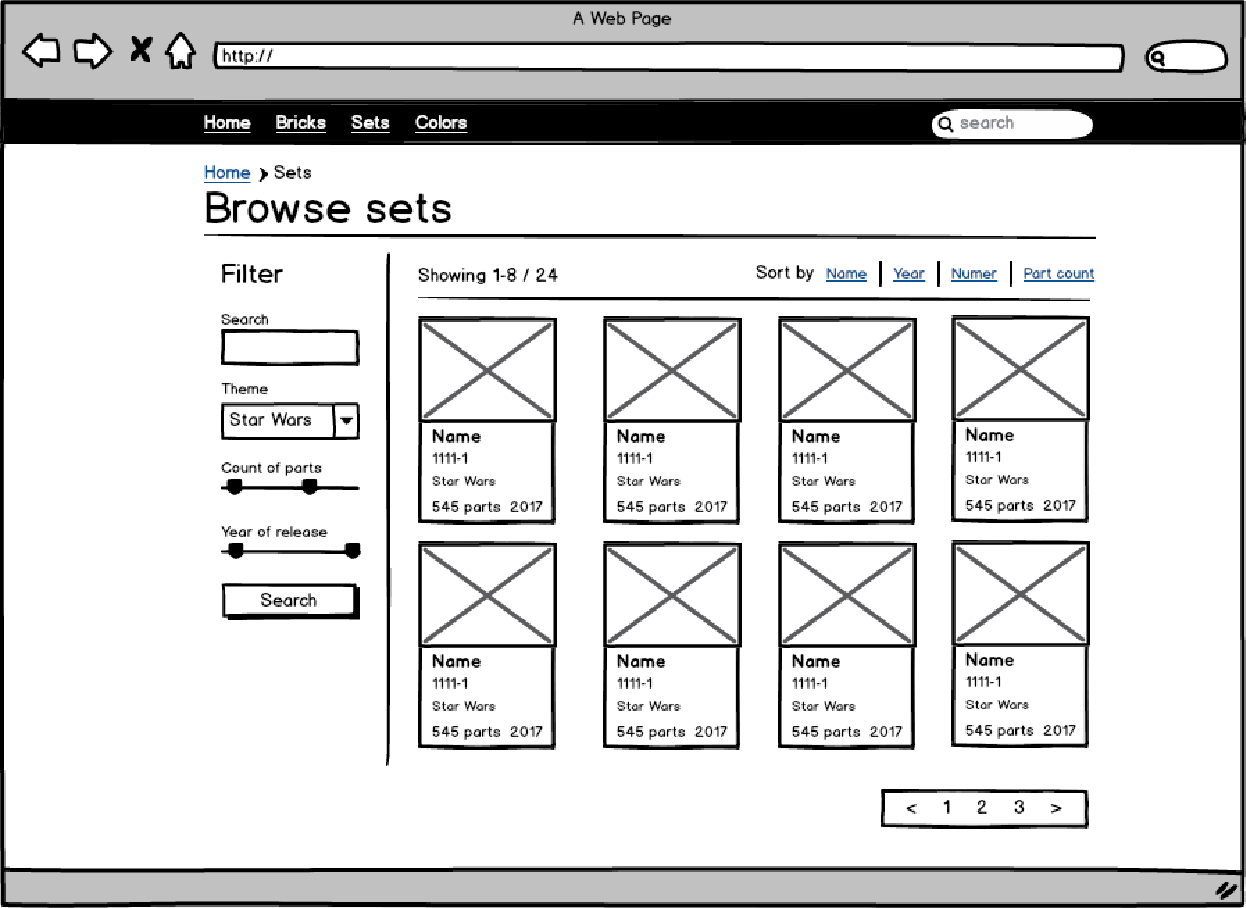
\includegraphics[width=\textwidth,height=\textheight,keepaspectratio]{pdfs/wireframe_sets.pdf}
    \caption{Návrh stránky výpisu stavebnic}\label{wireframe-stavebnice-seznam}
\end{figure}

\subsection{Výpis součástek}
Stránka výpisu součástek (obrázek \ref{wireframe-soucaska-seznam}) je rozložením prvků navržena stejně jako stránka výpisu stavebnic. 

\begin{figure}[htbp]
    \centering
    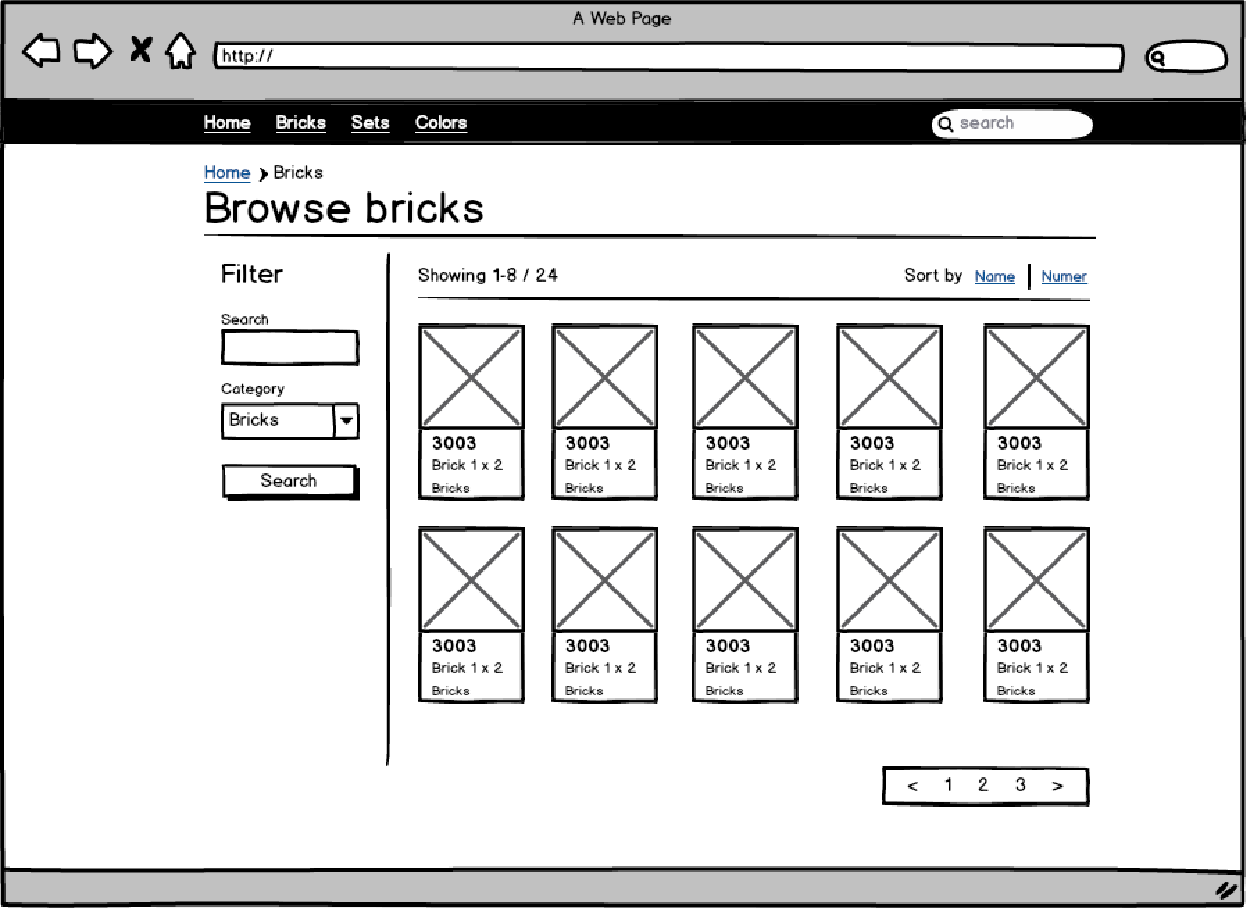
\includegraphics[width=\textwidth,height=\textheight,keepaspectratio]{pdfs/wireframe_bricks.pdf}
    \caption{Návrh stránky výpisu součástek}\label{wireframe-soucaska-seznam}
\end{figure}

\subsection{Detail stavebnice}
Stránka detailu stavebnice (obrázek \ref{wireframe-stavebnice-detail}) představuje uživateli veškeré dostupné informace o~stavebnici. Stránka je grafiky rozdělena na dva bloky. 

Hlavní blok obsahuje obrázek stavebnice a atributy zobrazené v~tabulce. Dále obsahuje odkazy na služby ze kterých pochází zobrazená data.

Druhý blok je pro lepší přehlednost rozdělen do podstránek, které je možné přepínat pomocí horizontálního menu. Výchozí podstránkou je výpis součástek obsažených ve stavebnici. Tento výpis je možné zobrazit jak ve variantě ignorující barvy součástek, tak ve variantě roztříděné podle barev. Každá z~těchto variant obsahuje tlačítko pro stažení 3D modelů součástek.

Pokud pro stavebnici nejsou dostupné 3D modely všech součástek, je na stránce zobrazeno varování. 

\begin{figure}[htbp]
    \centering
    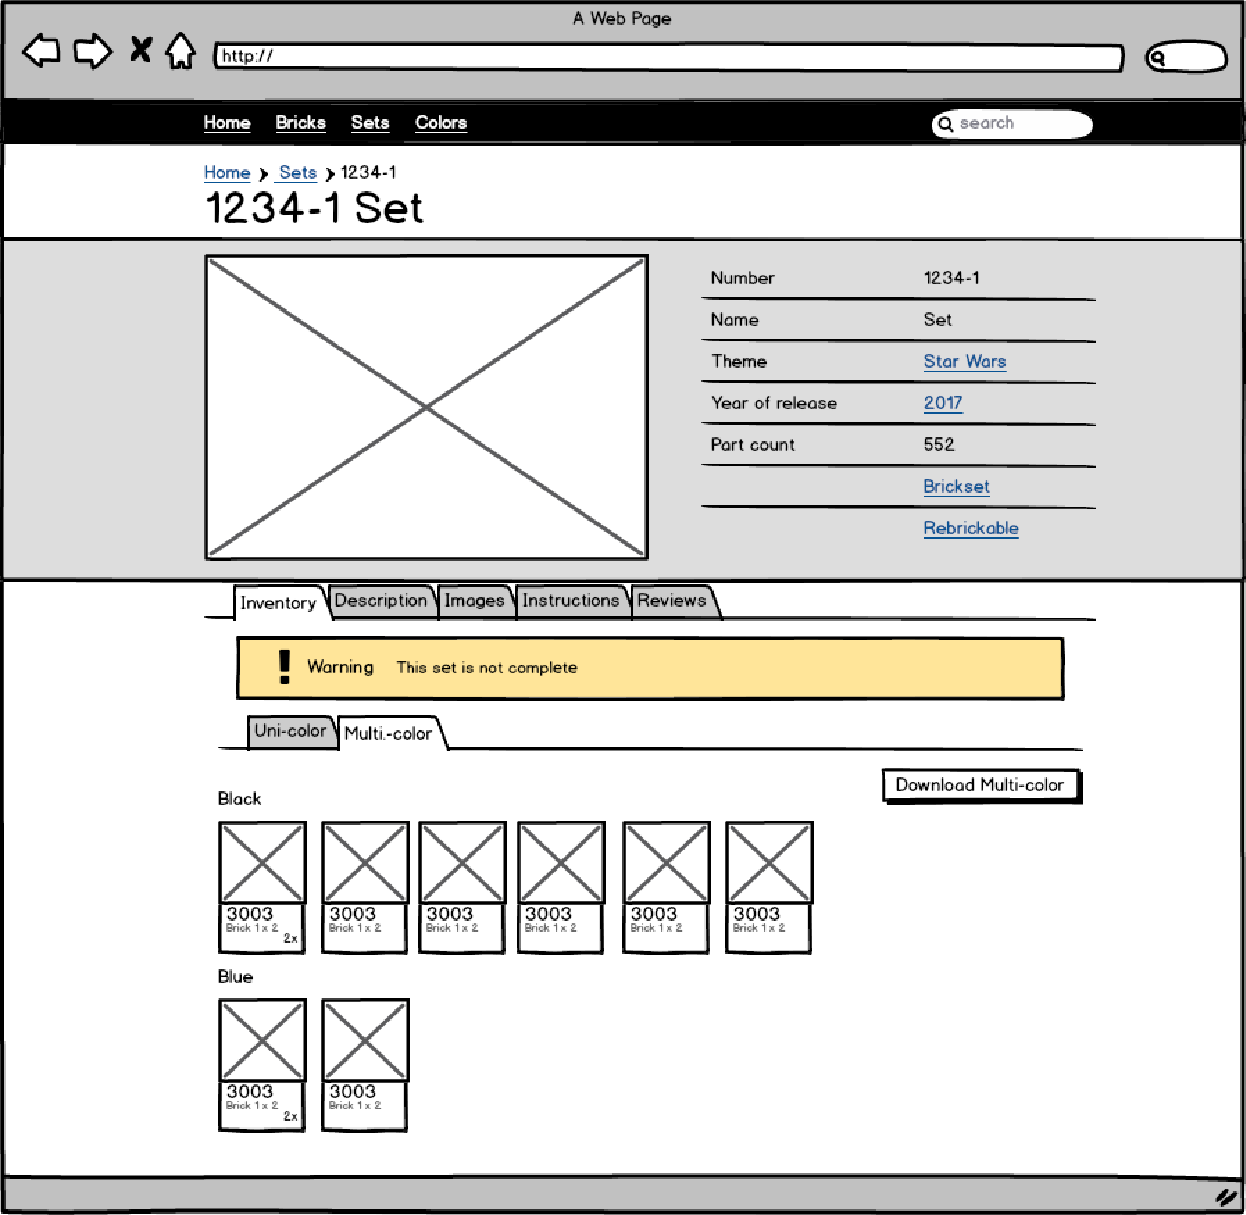
\includegraphics[width=\textwidth,height=\textheight,keepaspectratio]{pdfs/wireframe_set.pdf}
    \caption{Návrh stránky detailu stavebnice}\label{wireframe-stavebnice-detail}
\end{figure}

\subsection{Detail součástky}
Stránka detailu součástky (obrázek \ref{wireframe-soucastka-detail}) je navržena podobně jako stánka detailu stavebnice. 

Hlavní blok obsahuje obrázek součástky a přehled atributů. Obrázek součástky má v~pravém horním rohu tlačítko, kterým se spouští interaktivní 3D náhled. Dále blok obsahuje tlačítko pro stažení 3D modelu. 

Druhý blok obsahuje dvě podstránky. První podstránka zobrazuje všechny příbuzné součástky. V~druhé je možné prohlížet veškeré stavebnice, ve kterých se součástka vyskytuje.

\begin{figure}[htbp]
    \centering
    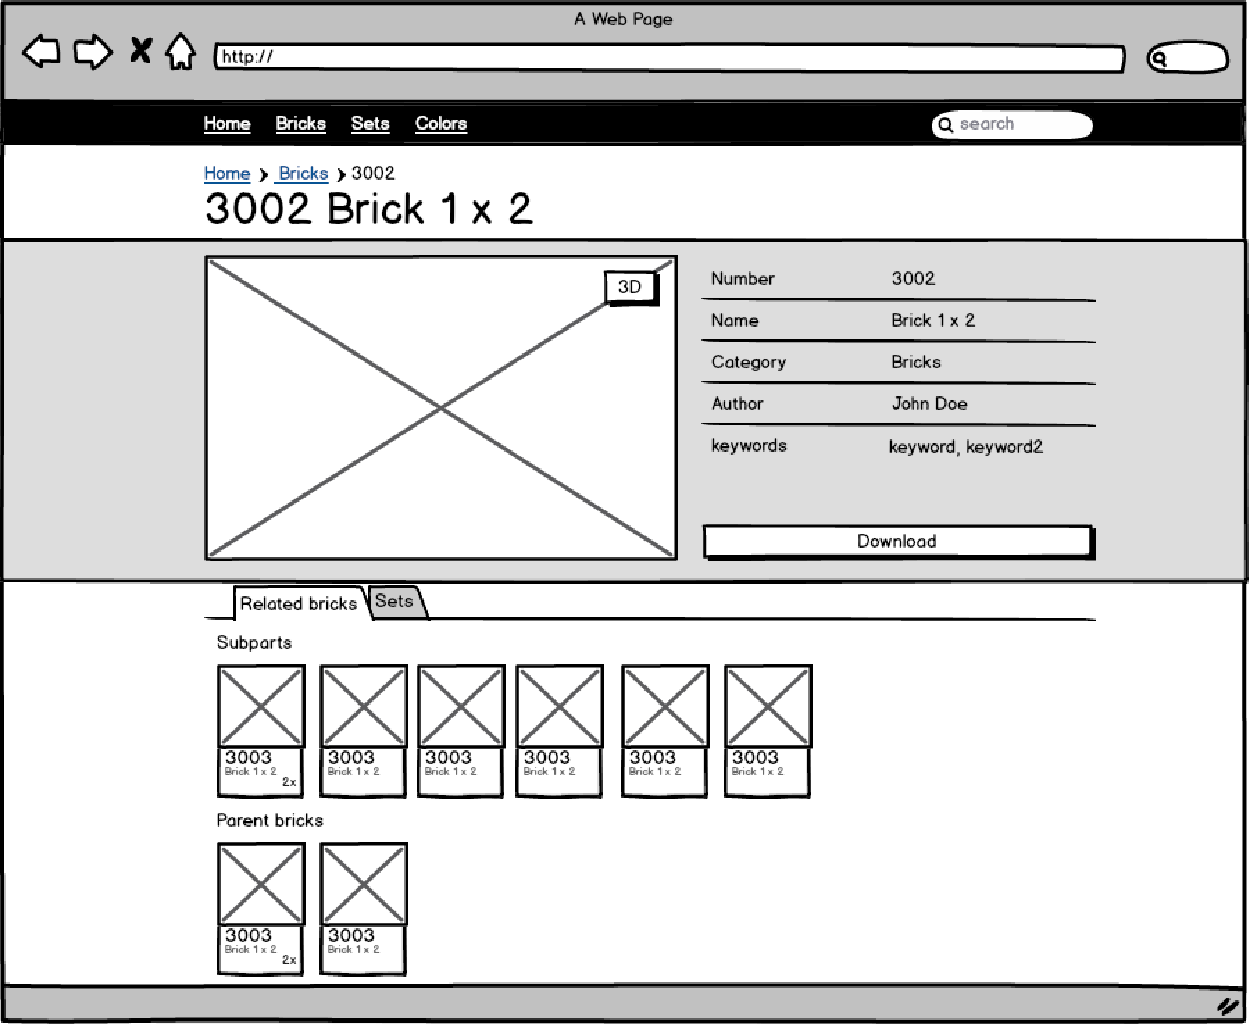
\includegraphics[width=\textwidth,height=\textheight,keepaspectratio]{pdfs/wireframe_brick.pdf}
    \caption{Návrh stránky detailu součástky}\label{wireframe-soucastka-detail}
\end{figure}

\subsection{Seznam barev}
Stránka seznamu barev (obrázek \ref{wireframe-barvy}) slouží uživatelům k~seznámení se s~možnými barevnými variantami součástek. Barvy jsou zobrazeny ve dvou tabulkách. První tabulka sdružuje klasické barvy a druhá transparentní barvy. 

\begin{figure}[htbp]
    \centering
    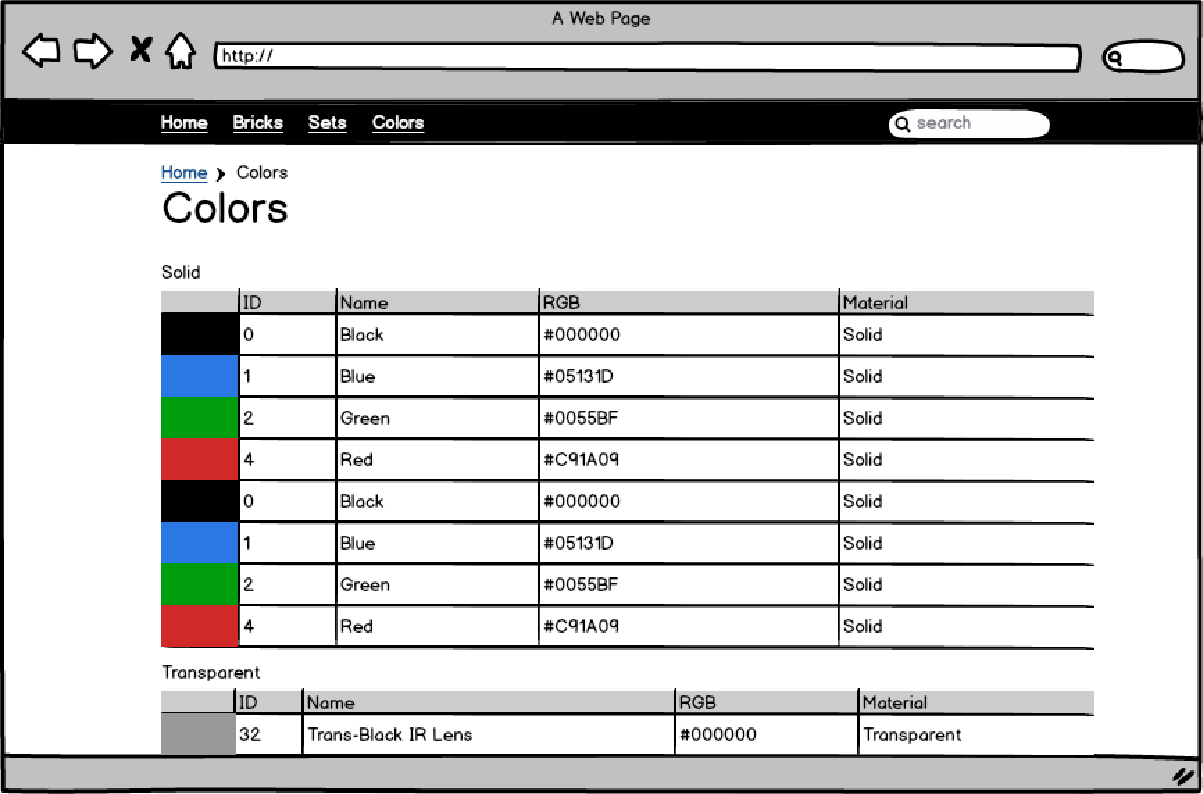
\includegraphics[width=\textwidth,height=\textheight,keepaspectratio]{pdfs/wireframe_colors.pdf}
    \caption{Návrh stránky seznamu barev}\label{wireframe-barvy}
\end{figure}